\providecommand{\main}{..}
\documentclass[main.tex]{subfiles}

\begin{document}
\chapter{Electronic Design}
\section{System Overview}

The electronic hardware of the system was designed according to the following principles, decided upon early in the project:
\begin{enumerate}
    \item The design shall be modular and will allow for adjustments in any stage of the design with minimal impact on the system as a whole.
    \item The design shall incorporate a general purpose, WiFi enabled companion computer.
    \item End-user input shall be limited to basic functionality, with no access to circuitry required for normal operation.
    \item The design shall incorporate verified circuitry where possible through the use of open-hardware COTS designs and application specific design tools.
\end{enumerate}
As a result of these, the final (1st generation) system took the form seen in \textit{Figure \ref{fig:electronics-system}}, featuring a Raspberry Pi Zero Wireless companion computer, stereo audio DAC, Class-D stereo amplifier, and several DC/DC power regulators. The required external connections were limited to a wall-mount 12V DC power supply, several buttons for user input, and a toggle switch to power the device.

\begin{figure}[H]
    \centering
    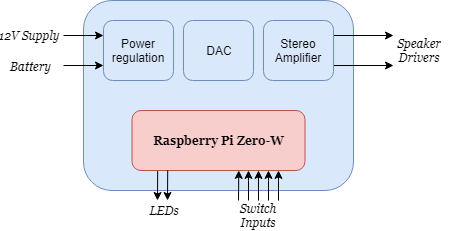
\includegraphics[scale=0.75]{./figs/electronics-system.png}        
    \caption{Electronics hardware overview}
    \label{fig:electronics-system}
\end{figure}

\section{Audio Stage}

On top of the system considerations, further requirements and desired features in the audio design were set early in the project:
\begin{itemize}
    \item The system shall utilise a Class-D audio amplifier (a remnant of the original project brief to design/build/test a 100W Class-D amplifier).
    \item The system shall be a bi-amp design, removing the requirement for hardware crossover filtering which shall instead be achieved through software. 
    \item The audio stage shall accept an $I^{2}S$ digital audio input from the companion computer and $I^{2}C$ communication for hardware control.
    \item Each driver shall have an amplification stage on the order of $\approx20W RMS$.
\end{itemize}

The resultant configurations from these requirements were then reduced to two choices: to have separated Digital-to-Analog conversion and Amplification stages, or to utilise a combined digital input amplifier, each presenting advantages and drawbacks.
\par
A fully integrated system presents both decreased BOM count and design effort - and greater immunity to noise - at the expense of setup requirements. Modern single-stage ICs offer far greater on-chip signal processing abilities but require a more sophisticated control scheme due to it, and often rely on expensive evaluation modules to ease their development. 
\par
A dual stage system is theoretically worse in signal integrity, and offers few advantages in this regard. In contrast to single stage systems, however, they provide far more choice in control complexity between each stage, and allow for the selection of ICs already in use within cheap COTS expansion modules. The advantage presented by this is the use of these COTS modules for software and audio development in parallel with electronic design, with the completed electronic system then seamlessly replacing the development setup upon completion.
\par
As both of these approaches offered interesting areas of investigation they were decided to be pursued in series. The initial system would utilise the advantages of the verified dual stage system and provide a guaranteed performance of the final system. The single stage system would then be developed afterwards with a lower priority, and would present room for comparison between the classical and modern design methodologies. To reduce complexity in the overall design and board bring-up components were selected such that each of the systems would have identical power stages and overall board design.

\subsection{1st Generation Dual-Stage Board}

The initial system designed can be seen in \textit{Figure \ref{fig:audio-system}}, with components selection governed by the availability of compatible COTS modules. 

\begin{figure}[H]
    \centering
    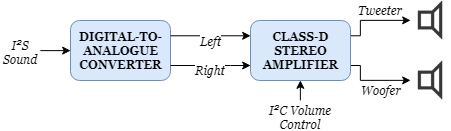
\includegraphics[scale=0.75]{./figs/audio-system.png}
    \caption{Dual stage audio system}
    \label{fig:audio-system}
\end{figure}

\subsubsection{DAC}
The initial module selected for development of the streaming software was the Pimoroni pHAT DAC, based on the Texas Instruments PCM5102A audio stereo DAC. This board not only met the hardware requirements, but as a dedicated expansion board for the Pi Zero W provided device tree setup and software libraries which expedited testing. The board layout and component choice both conformed to the recommended application information provided within the component datasheet, and thus could be reliably replicated, as seen in \textit{Figure \ref{fig:dac-circuit}}.

\begin{figure}[H]
    \centering
    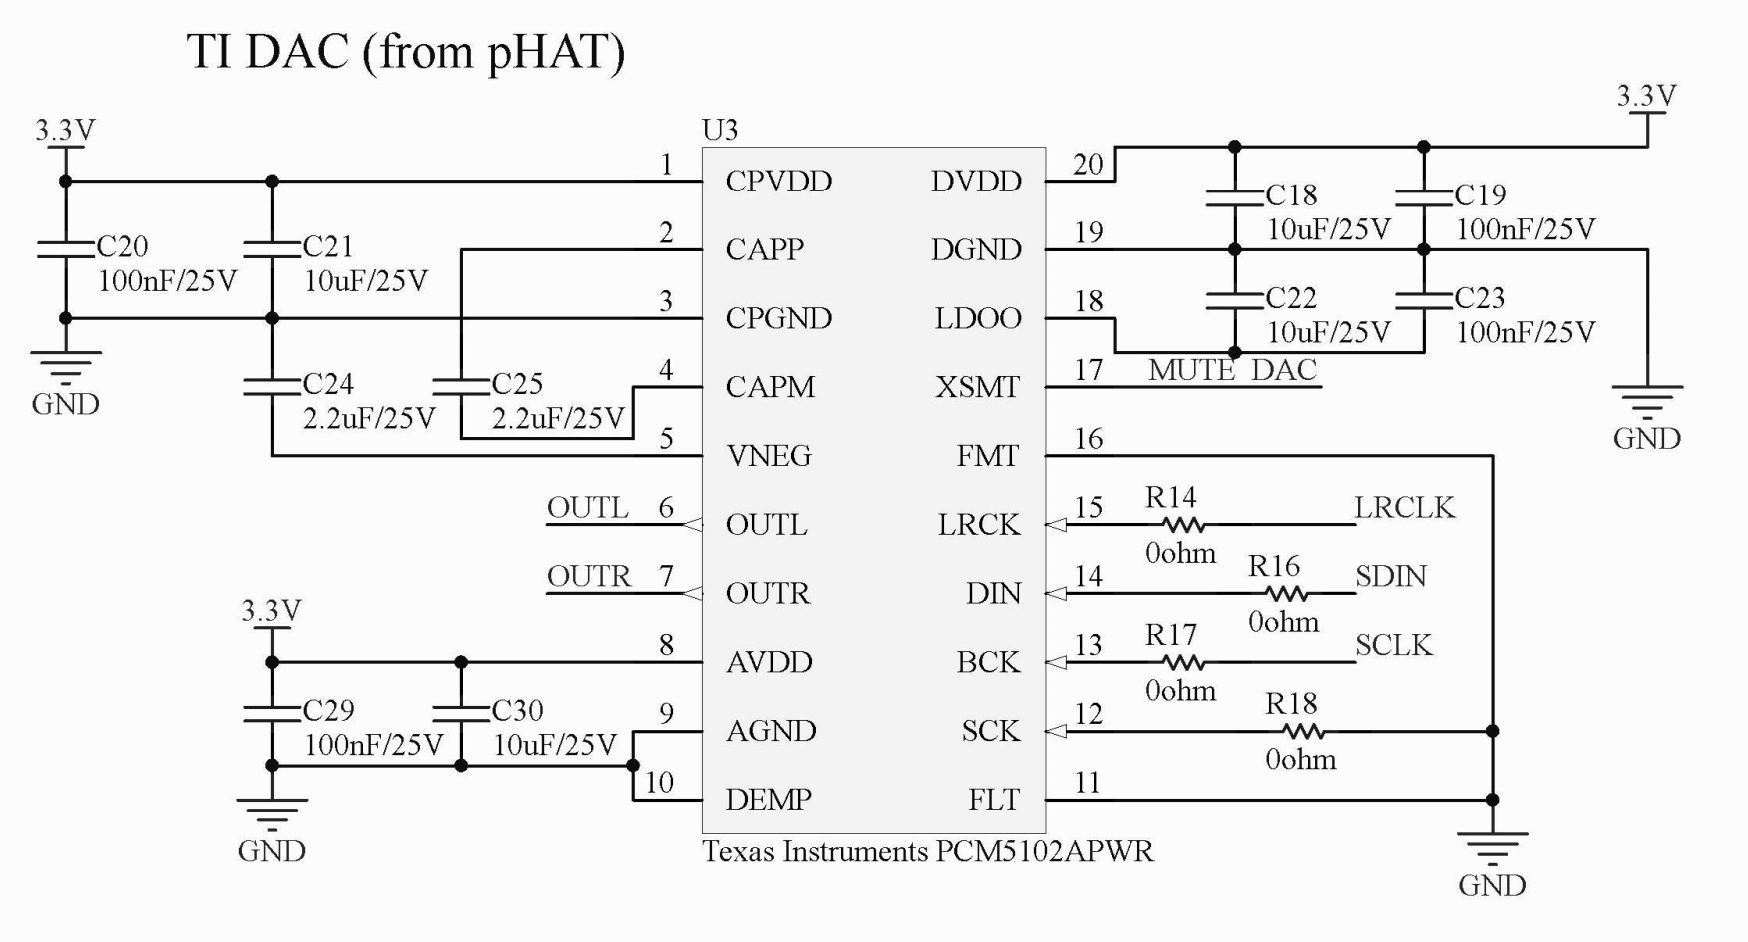
\includegraphics[scale=0.6]{./figs/DAC-circuit.PNG}
    \caption{DAC schematic}
    \label{fig:dac-circuit}
\end{figure}

\subsubsection{Amplifier}
The amplifier stage selection was governed by the desire for low control complexity and low BOM cost while maintaining the aforementioned requirements. The Maxim Integrated MAX9744 fit these criteria with the advantage of its use in a range of commercial designs. The required control is limited to the volume selection by setting a single register value, and its capability to use ferrite beads on its outputs removed the significant cost power inductors present to class-d design. As shown in \textit{Figure \ref{fig:maxim-circuit}}, the recommended schematics and layouts provided in the device datasheet were again used. Hardware analog control was disabled and 100nF decoupling capacitors added alongside the bulk capacitance on the power supply pins.

\begin{figure}[H]
    \centering
    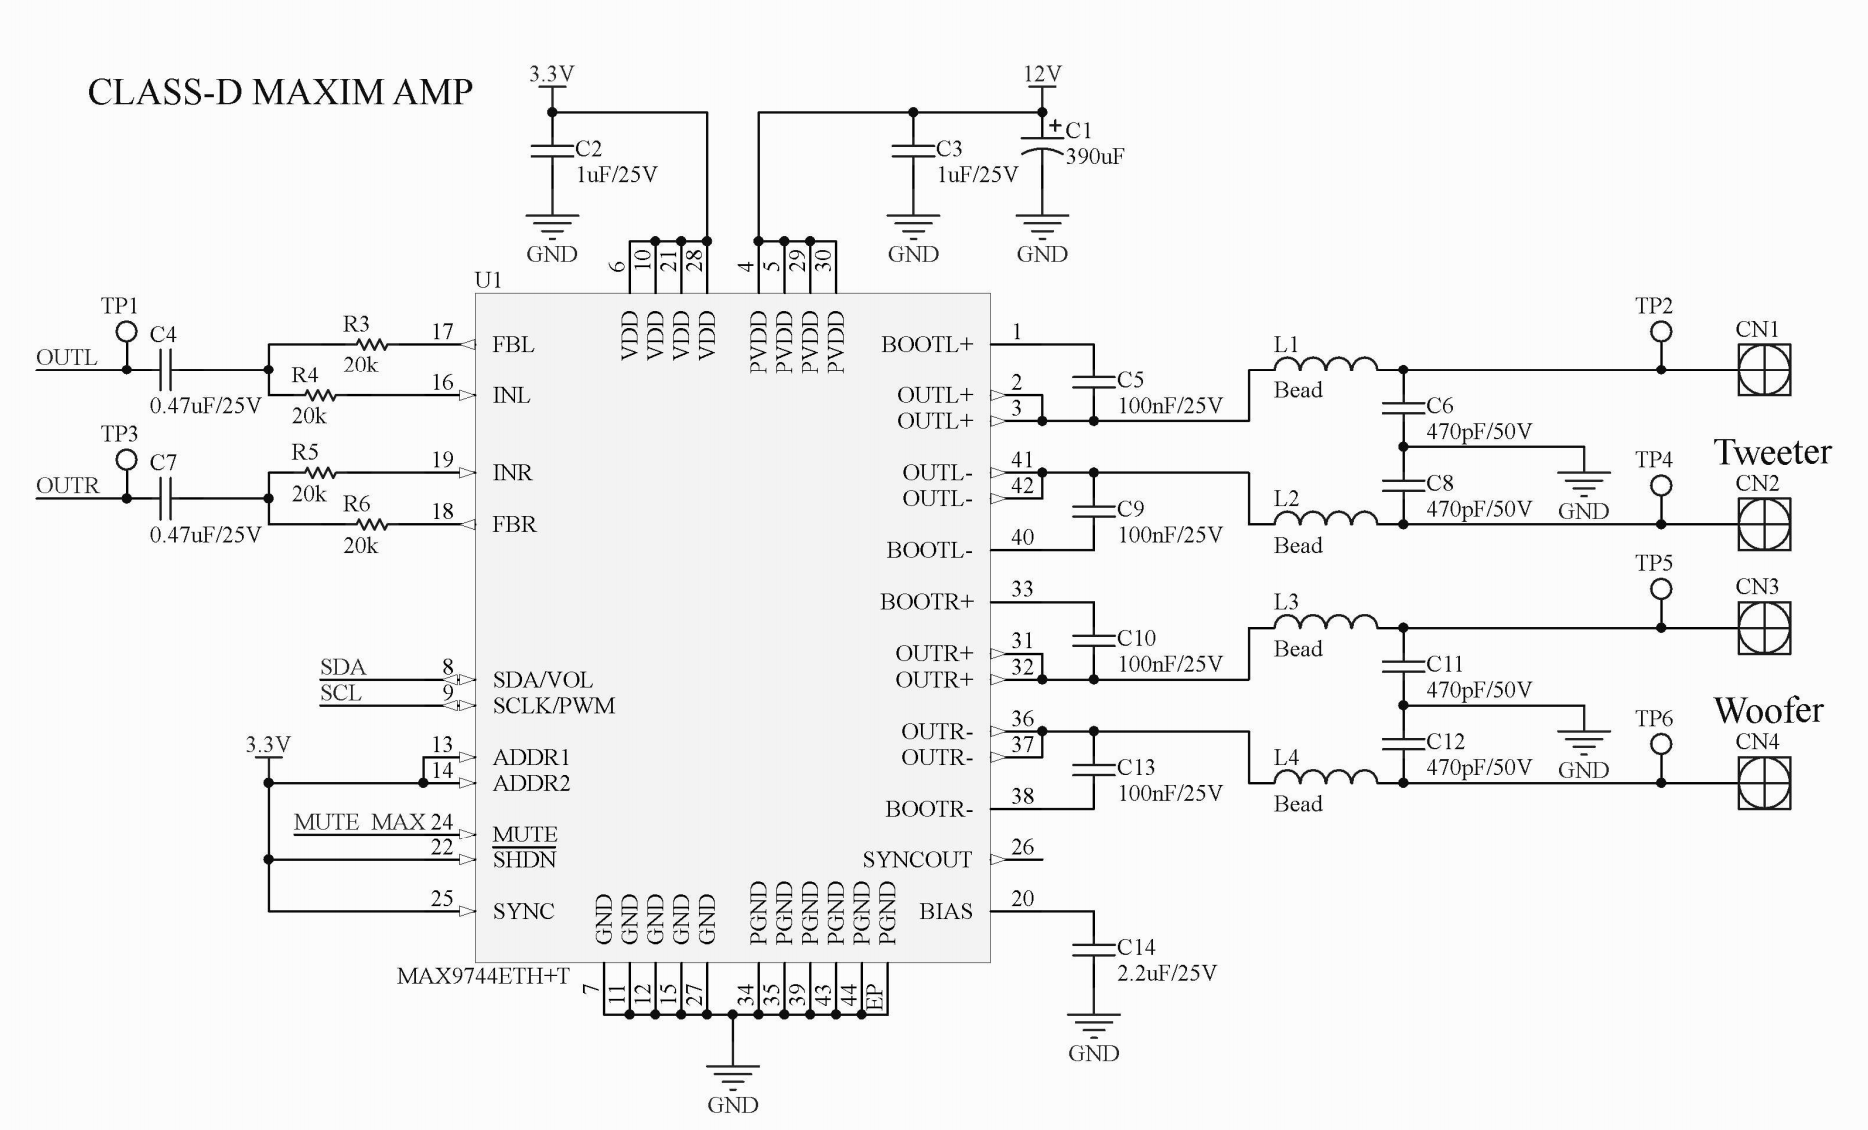
\includegraphics[scale=0.6]{./figs/MAXIM-circuit.PNG}
    \caption{Amplifier schematic}
    \label{fig:maxim-circuit}
\end{figure}

\subsection{2nd Generation Single-Stage Board}

\begin{figure}[H]
    \centering
    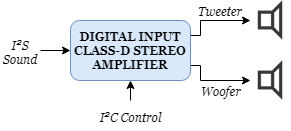
\includegraphics[scale=0.75]{./figs/TAS-system.png}
    \caption{Single stage audio system}
    \label{fig:tas-system}
\end{figure}

For subsequent development of the fully integrated system a digital input amplifier was selected based on its conformance to the project requirements as well as the previously generated power supply. The result of this was the Texas Instruments TAS5805M, a far more modernised IC than those in the dual system capable of accepting the same $I^S$ signal and $I^2C$ control signals while incorporating a wealth of DSP capabilities. The produced schematic can be seen in \textit{Figure \ref{fig:tas-circuit}} and worked as desired barring the lack of address-setting resistor due to an error in design.

\begin{figure}[H]
    \centering
    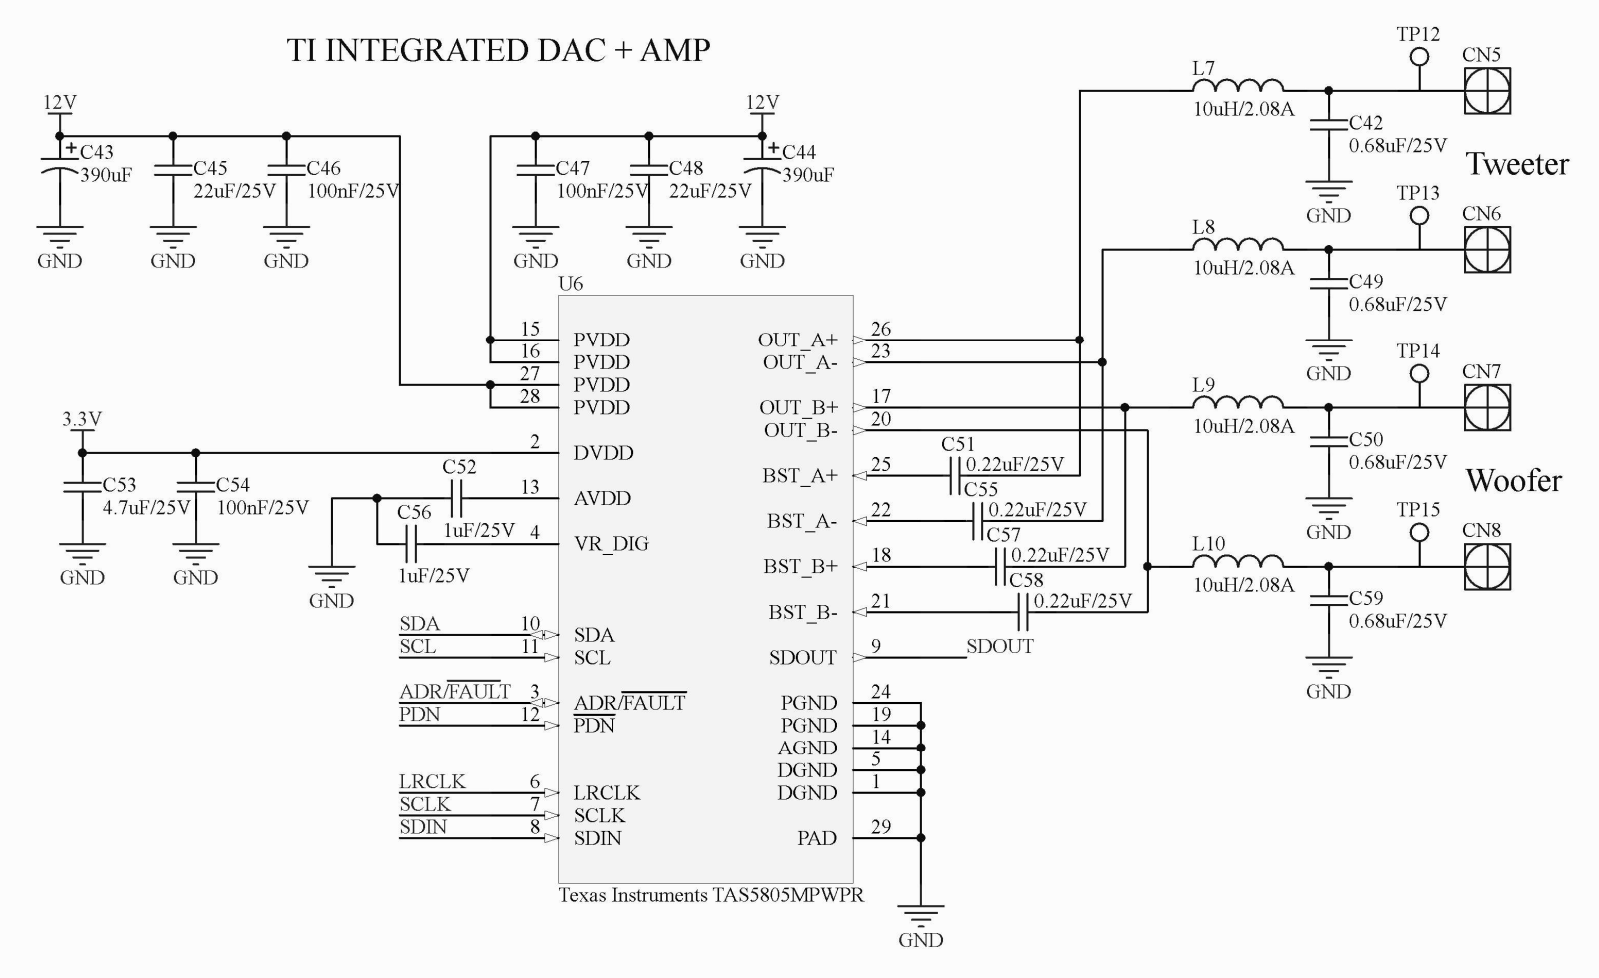
\includegraphics[scale=0.75]{./figs/TAS-circuit.PNG}
    \caption{Digital input amplifier schematic}
    \label{fig:tas-circuit}
\end{figure}

While development without an evaluation module presented a challenge, the initial configuration of the device was still able to be achieved through use of the Texas Instruments PurePath Configurator 3 software package. This was used to generate configuration header files as an array of $I^2C$ addresses and commands, providing the required register values as well as page navigation of the device.

\section{Power Stage}

To power the system three regulated outputs were required. The amplifier power inputs were supplied by a 12V rail, a 5V rail powered the companion computer, and a final 3.3V supply provided the logic level power for the board ICs. The system was then selected utilising the Texas Instrument Webench power designer, prioritising for low BOM cost and footprint area. Two TI TPS62135 buck regulating DC/DC converters were chosen to generate the 12V (from unregulated battery power) and 5V high current rails, with a TI TLV70033 LDO regulator provided the low power logic level supply. 

\begin{figure}[H]
    \centering
    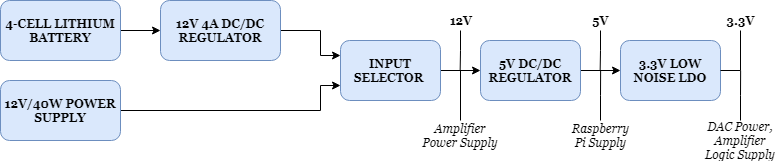
\includegraphics[scale=0.6]{./figs/power-system.png}
    \caption{Power regulation electronics}
    \label{fig:power-system}
\end{figure}

To avoid the risk presented by mains power regulation the speakers were designed such that the user faced only a 12V $\approx$ 40W power supply that could be sourced from a validated supplier. This was chosen as the XP Power VEL36US120-UK-JA, a generic COTS supply fit for the purpose which, while being rated only for 36W, fit the desired form factor and cost requirements enough to be seen as an acceptable risk.

\begin{figure}[H]
    \centering
    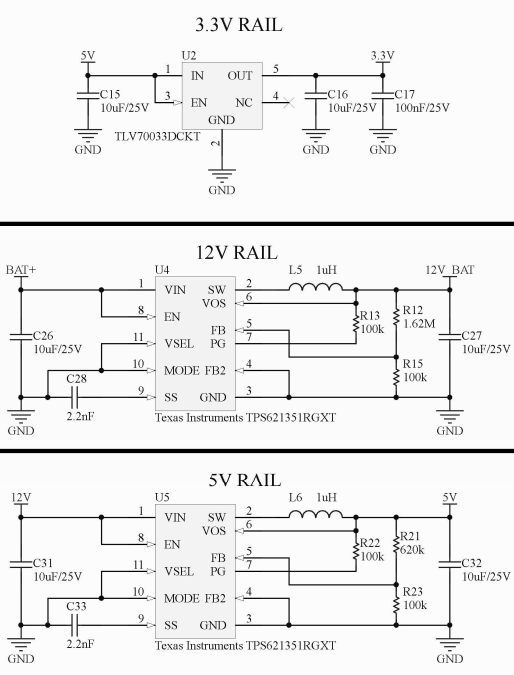
\includegraphics[scale=1.2]{./figs/power-circuit.PNG}
    \caption{Power regulation schematic}
    \label{fig:power-circuit}
\end{figure}

\subsubsection{Design Considerations}

Although the system design was largely governed by the Webench designer and datasheet applications small changes were made to the system to incorporate good-practice procedures. Power inputs and outputs on each subsystem were decoupled with 100nF transient suppressing capacitors as well as a local bulk capacitance. Any MLCCs (multi-layer ceramic capacitors) used were rated for 25V to mitigate the large derating seen well below their advertised rated voltage, and extra footprints for bulk capacitance were placed around the board. 

\subsection{Battery Power}

To incorporate the desire for the system to operate in a truly wireless sense circuitry was added to handle the selection and regulation of a 4-cell lithium-polymer battery power supply. A P-type FET placed in series with the regulated battery output switched the supply off based on the insertion of the DC barrel jack and vice-versa. As this use case of the system was only for test and not a feature of the device, protection and charging circuitry was not provided. A future design may implement these, and would replace the COTS protected battery with several 18650 cells and appropriate voltage and charging protection.

\section{PCB Design}

Schematic capture and PCB design were both handled in Altium's community oriented Circuitmaker software. Components were selected based on their availability at preferred suppliers - namely Onecall - and selected in the design using the platform's OCtopart component database integration. This method allowed for both the use of community generated footprints as well as the generation of supplier specific BOMs for purchasing. 

\subsection{Test Boards}
To allow for design verification and early testing PCBs were fabricated containing each of the audio stages. Power supplies were left off the board and each was built to simply attach as a shield to the companion computer, as seen in \textit{Figure \ref{fig:ti-pcb}}.

\begin{figure}[H]
    \centering
    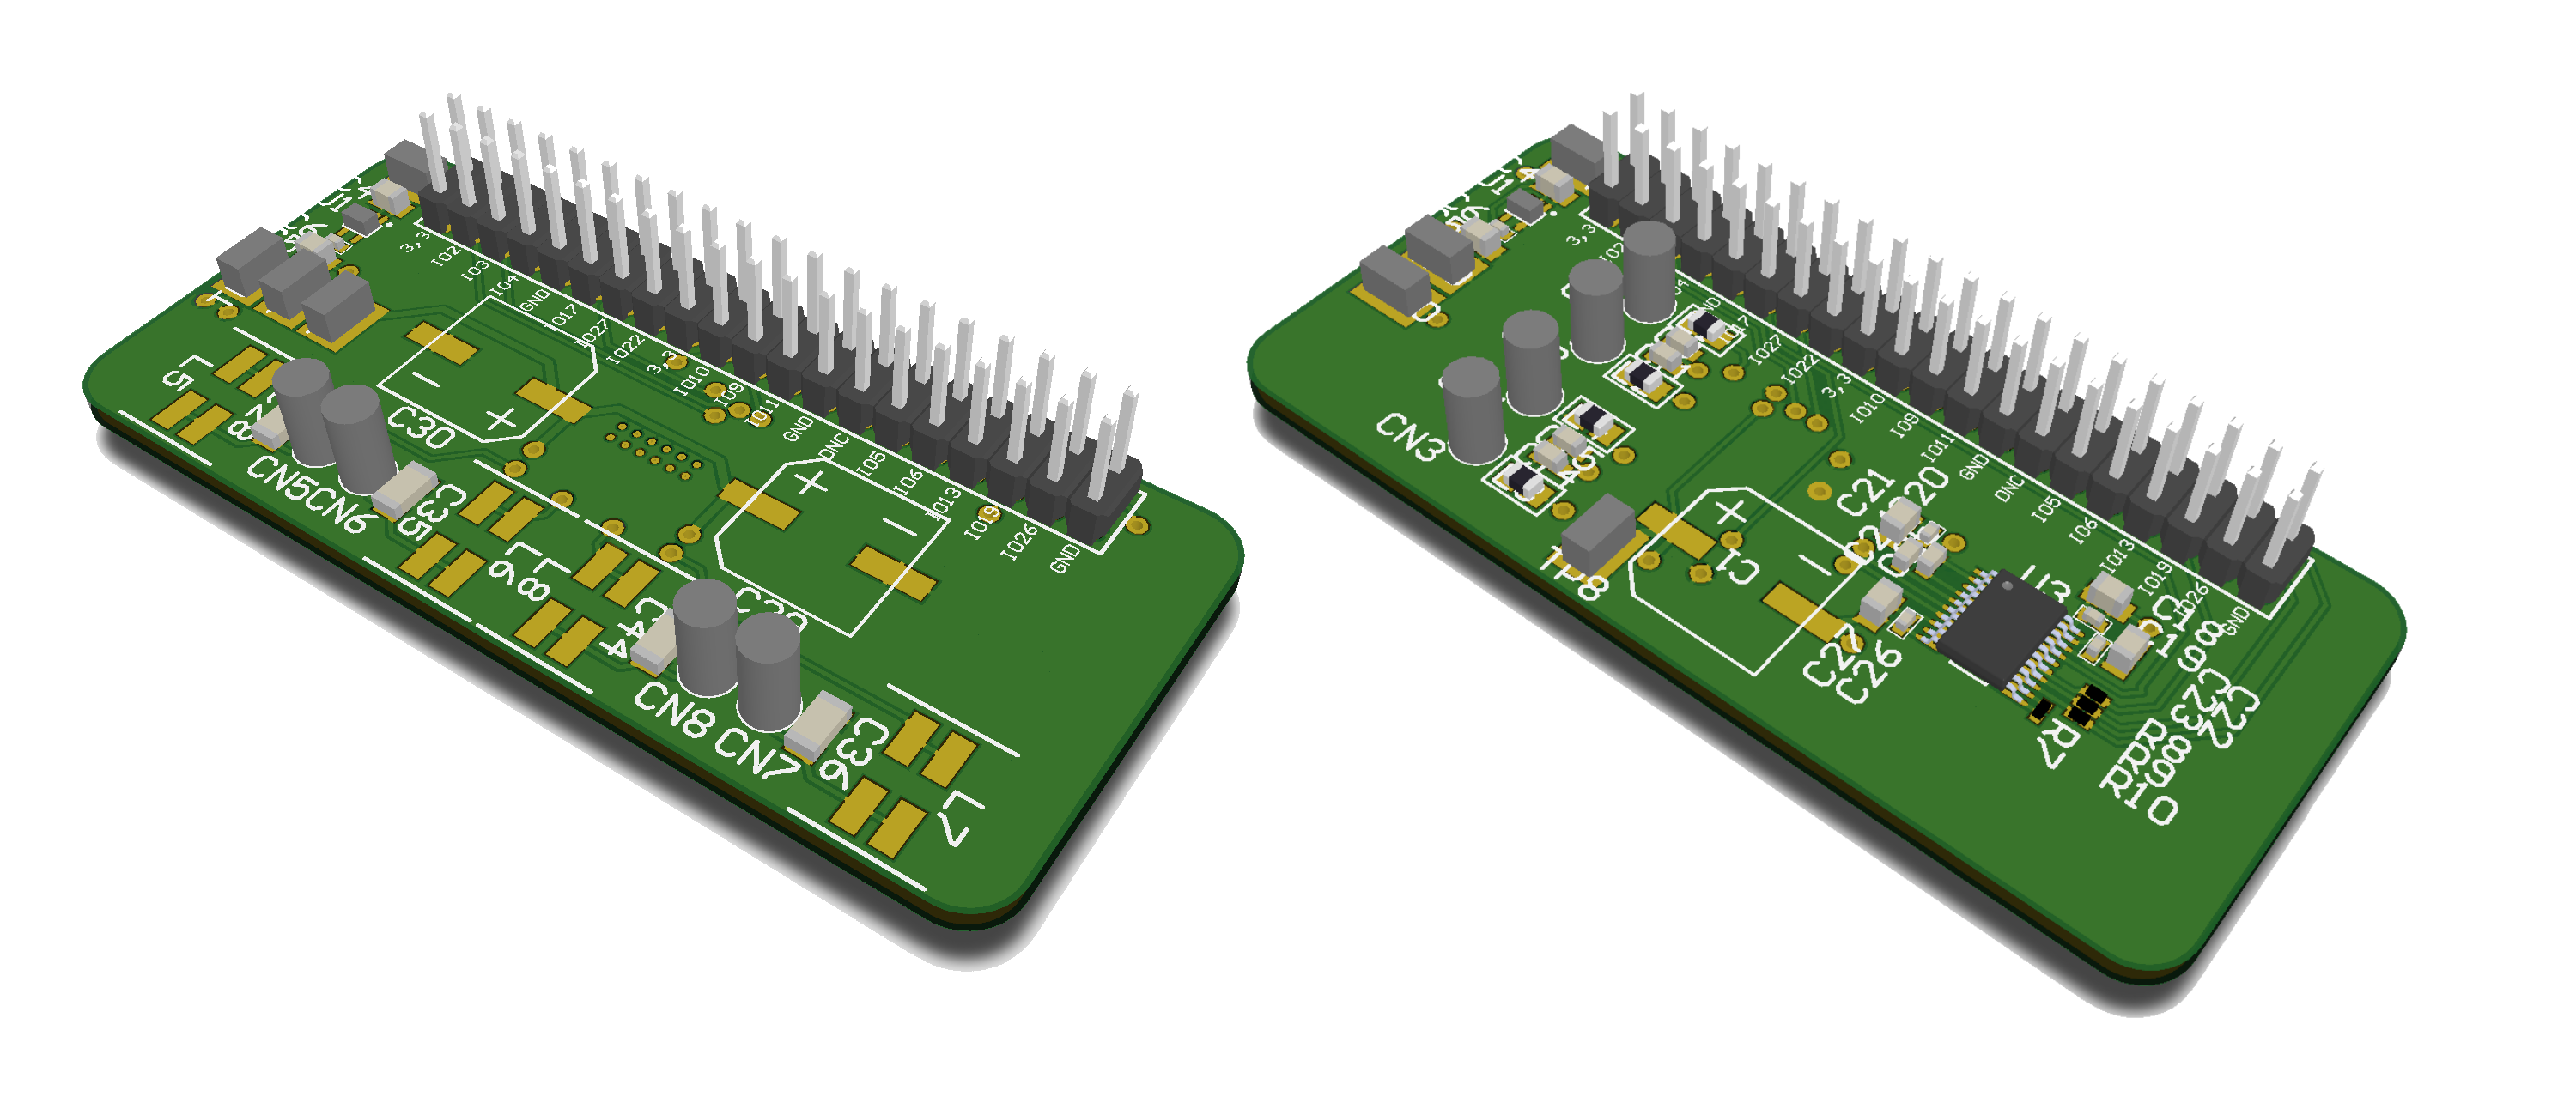
\includegraphics[scale=0.2]{./figs/test-boards.png}
    \caption{Audio test boards}
    \label{fig:ti-pcb}
\end{figure}

\subsubsection{Layout}

Placement of components and passives closely followed the recommended layouts given in their datasheets, with each block placed into its respective audio, power, or debug board regions. Signal traces were kept to 10mil widths, with a ground and 12V plane poured over the top and bottom of the board respectively. 

\begin{figure}[H]
    \centering
    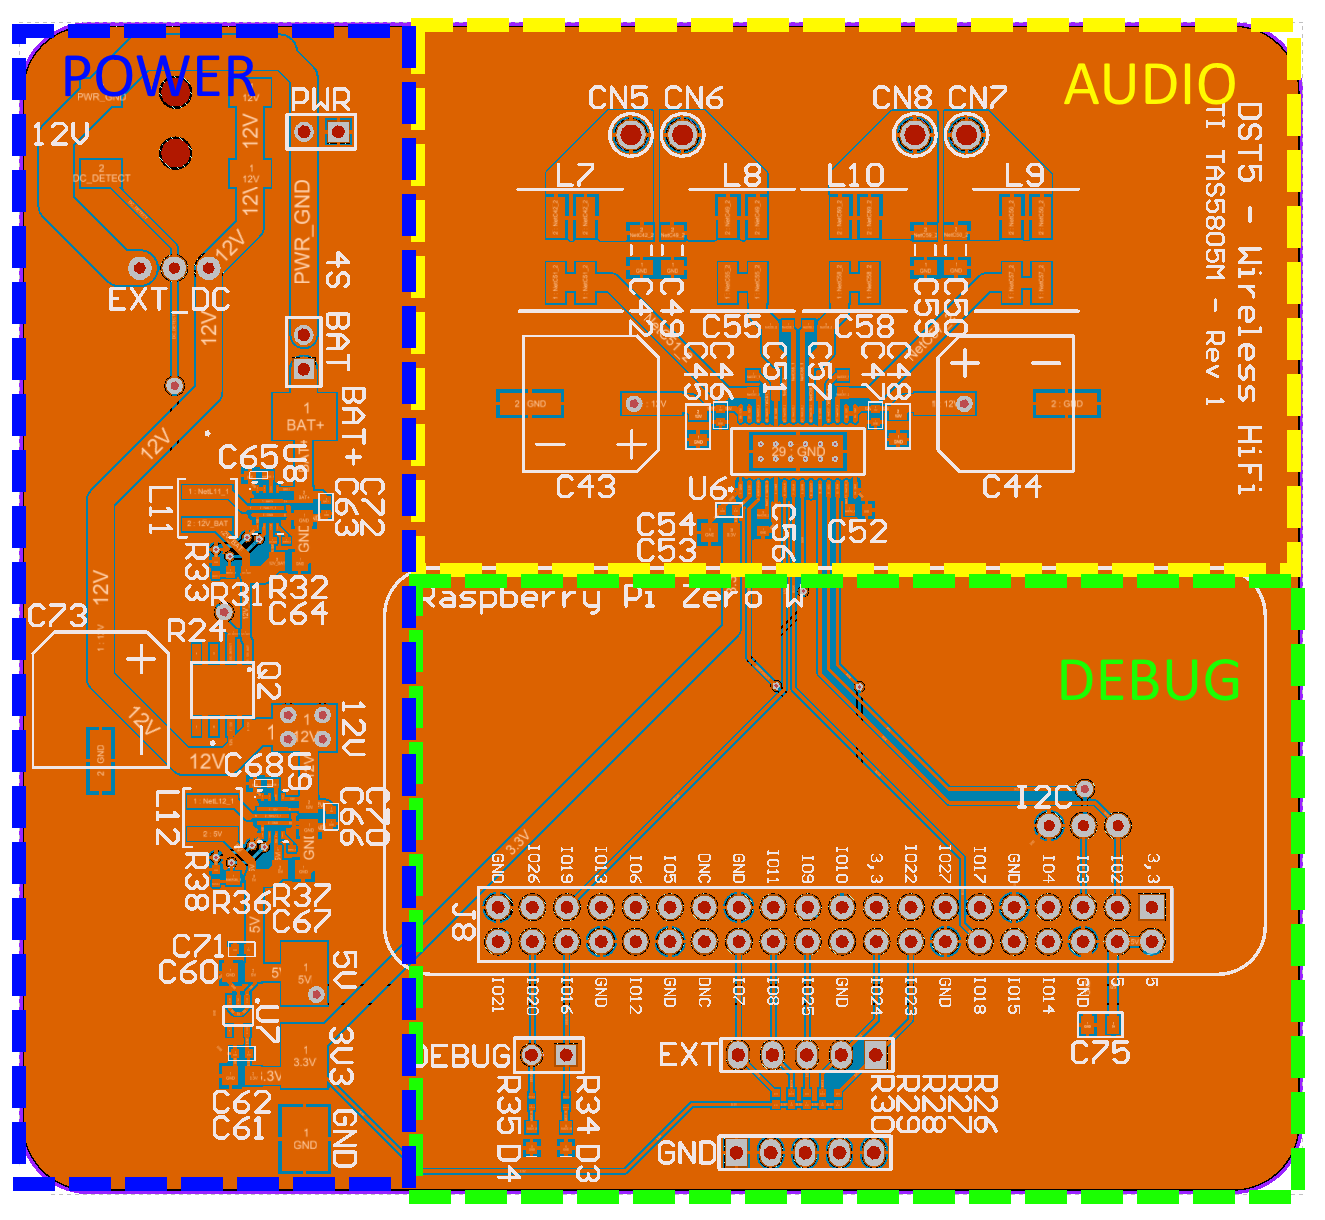
\includegraphics[scale=0.4]{./figs/ti-pcb.png}
    \caption{Single stage board layout}
    \label{fig:ti-pcb}
\end{figure}

\subsubsection{Fabrication}

While the initial test boards were produced in-house by university technicians, the scale of many surface mount components and number of vias in the design prohibited this in the final product. The boards were therefore manufactured externally, with soldermask and silkscreen added to ease production as seen in \textit{Figure \ref{fig:ti-board}}. 

\begin{figure}[H]
    \centering
    \includegraphics[scale=0.15]{./figs/ti-board.png}
    \caption{Populated single stage board}
    \label{fig:ti-board}
\end{figure}

\section{User I/O}
As the internals of the system were not intended to be user-facing, adequate controls had to be brought out of the cavity to allow for essential user input. 
\subsubsection{Tactile Switches}
Three tactile switches - mounted on padboard - were connected to the external switch pins on the main PCB with ribbon cable. Glued to each was a 12mm 3D printed spacer, which then protruded through three corresponding holes in the back of the enclosure. These were then programmed to act as volume up, volume down, and soft power-down for the raspberry pi (preventing potential data corruption from a hard shutdown of the companion PC).
\subsubsection{Power Supply}
The only required connection to the device is that for a 12V wall power supply, and thus only required a panel mount 5.5x2.1mm barrel jack receptacle. This was then placed in series with a SPDT toggle switch to act as a hardware power control, and holes for each drilled in the back plate of the enclosure.

\section{Testing}
\subsection{Overview}
The core evaluation of audio electronics requires the measurement of both the noise and harmonic loss between the input and output stage. For the dual stage system this occurs at two places: the inherent quantisation of the DAC output, and the noise introduced within the amplifier. The combined measurement of these effects is dubbed the Total Harmonic Distortion + Noise, and can be measured with a variety of equipment. In the absence of a specialised test setup, a rudiment measurement was achieved using a digital storage oscilloscope with a \textit{Fast Fourier Transform} function as such:

\begin{itemize}
    \item A 1kHz sine wave was output from the raspberry pi across the I2S lines.
    \item A Keysight DSOX1102G oscilloscope probe was connected across the amplifier/DAC output and set to 10ms/division with appropriate voltage scaling.
	\item A FFT function was applied to the channel under test, with a span of 20kHz and centre frequency of 10kHz.
	\item A sample of the FFT data was recorded with and without the input sine wave.
	\item The area under the resultant trace is integrated to give the fundamental signal strength across the audible range.
	\item A notch filter was applied to remove the 1kHz sine wave from the frequency response and the area under the new curve integrated.
	\item The ratio of the signal strength without the desired sine wave versus the fundamental signal strength is taken, and the resultant value taken as the THD+N of the output signal.
	\item Alternatively, by importing the FFT spectrum to MATLAB, the thd() function may be used to select the fundamental frequency and calculate the system THD without noise by integrating only the signal harmonics. 
\end{itemize}


\subsection{Results}

The resultant FFT traces of the following signals are shown below, along with the resultant THD values via MATLAB. For comparison, the THD of the DAC was also measured using a Voltech PM1000+ power analyser and given as 0.36\%. Due to the speciality of this test equipment its value was assumed to be known good, however, due to its primary goal being for analysis of power line frequencies, it was not applicable to the class-d output of the amplifiers.
\par

\begin{center}
\begin{tabular}{c|c|c}
    System & THD(dB) & THD(\%) \\
    \hline
    DAC & -52.58 & 0.2349633 \\
    MAXIM9744 & -17.67 & 13.0767554 \\
    TAS5805M & -35.33 & 1.7119852 \\
\end{tabular}
\end{center}

\begin{figure}[H]
    \begin{tikzpicture}
        \begin{axis}[
            width=\textwidth, 
            height=\axisdefaultheight,  
            xlabel={Frequency},
            ylabel={Gain(dB)},  
            xmin=0,
            xmax=20000,     
        ]
        %\addplot table [mark=none, x=t, y=a, col sep=comma] {./data/saleae-outputs/sync.csv};
        
        \addplot table [mark=none, x=f, y=a, col sep=comma] {./data/csvs/test_001_1.csv};
        \end{axis}
    \end{tikzpicture}
    \caption{Raw FFT of MAX9744 (no input) from Scope}
    \label{fig:lowpass-fft}
\end{figure}

\begin{figure}[H]
    \begin{tikzpicture}
        \begin{axis}[
            width=\textwidth, 
            height=\axisdefaultheight,  
            xlabel={Frequency},
            ylabel={Gain(dB)},  
            xmin=0,
            xmax=20000,     
        ]
        %\addplot table [mark=none, x=t, y=a, col sep=comma] {./data/saleae-outputs/sync.csv};
        
        \addplot table [mark=none, x=f, y=a, col sep=comma] {./data/csvs/test_001_3.csv};
        \end{axis}
    \end{tikzpicture}
    \caption{Raw FFT of MAX9744 (1kHz sine input) from Scope}
    \label{fig:maxim-thd}
\end{figure}

\begin{figure}[H]
    \begin{tikzpicture}
        \begin{axis}[
            width=\textwidth, 
            height=\axisdefaultheight,  
            xlabel={Frequency},
            ylabel={Gain(dB)},  
            xmin=0,
            xmax=20000,     
        ]
        %\addplot table [mark=none, x=t, y=a, col sep=comma] {./data/saleae-outputs/sync.csv};
        
        \addplot table [mark=none, x=f, y=a, col sep=comma] {./data/csvs/test_001_4.csv};
        \end{axis}
    \end{tikzpicture}
    \caption{Raw FFT of PCM5102A (no input) from Scope}
    \label{fig:dac-fft}
\end{figure}

\begin{figure}[H]
    \begin{tikzpicture}
        \begin{axis}[
            width=\textwidth, 
            height=\axisdefaultheight,  
            xlabel={Frequency},
            ylabel={Gain(dB)},  
            xmin=0,
            xmax=20000,     
        ]
        %\addplot table [mark=none, x=t, y=a, col sep=comma] {./data/saleae-outputs/sync.csv};
        
        \addplot table [mark=none, x=f, y=a, col sep=comma] {./data/csvs/test_001_5.csv};
        \end{axis}
    \end{tikzpicture}
    \caption{Raw FFT of PCM5102A (1kHz sine input) from Scope}
    \label{fig:dac-thd}
\end{figure}

\begin{figure}[H]
    \centering
    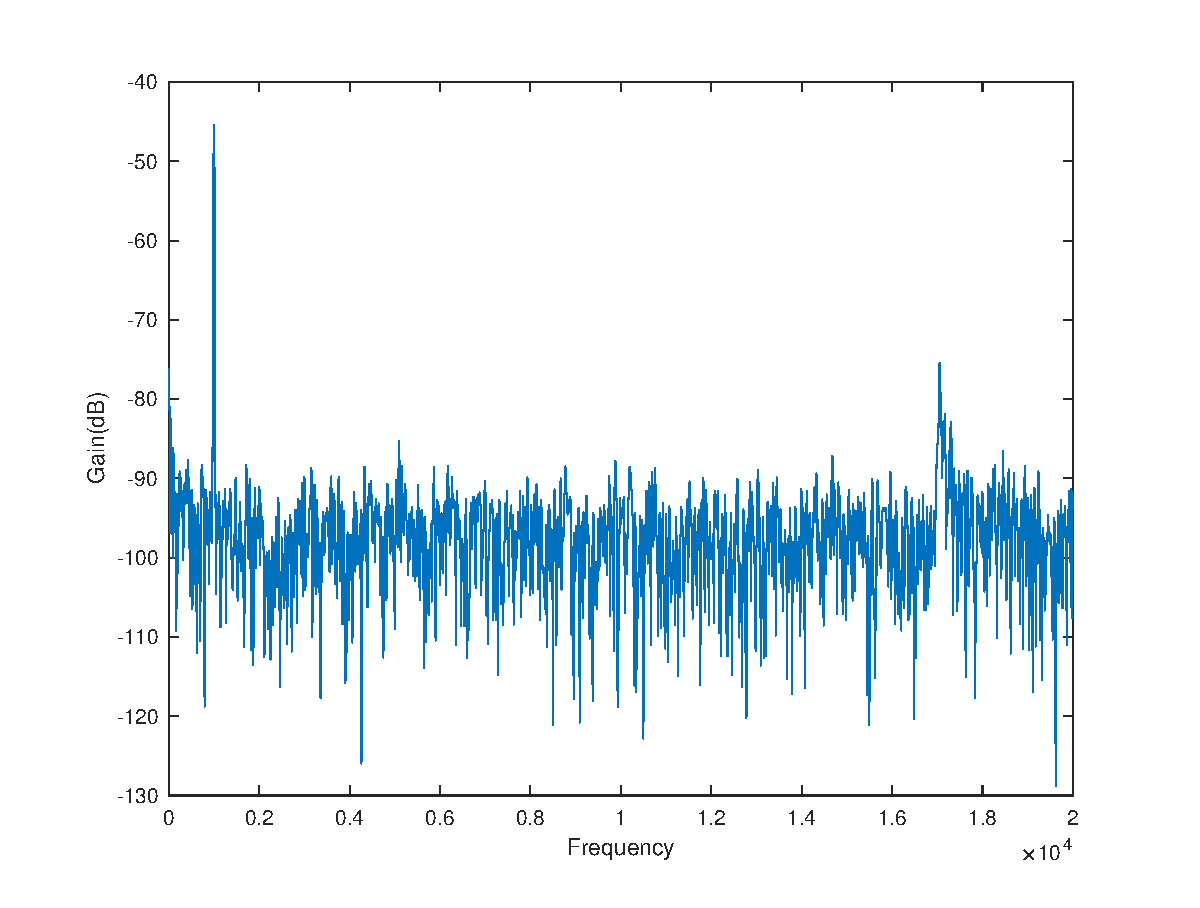
\includegraphics[scale=0.75]{./figs/TI_THD.eps}        
    \caption{Raw FFT of TAS5805M (1kHz sine input) from Scope}
    \label{fig:ti-thd}
\end{figure}

\begin{figure}[H]
    \centering
    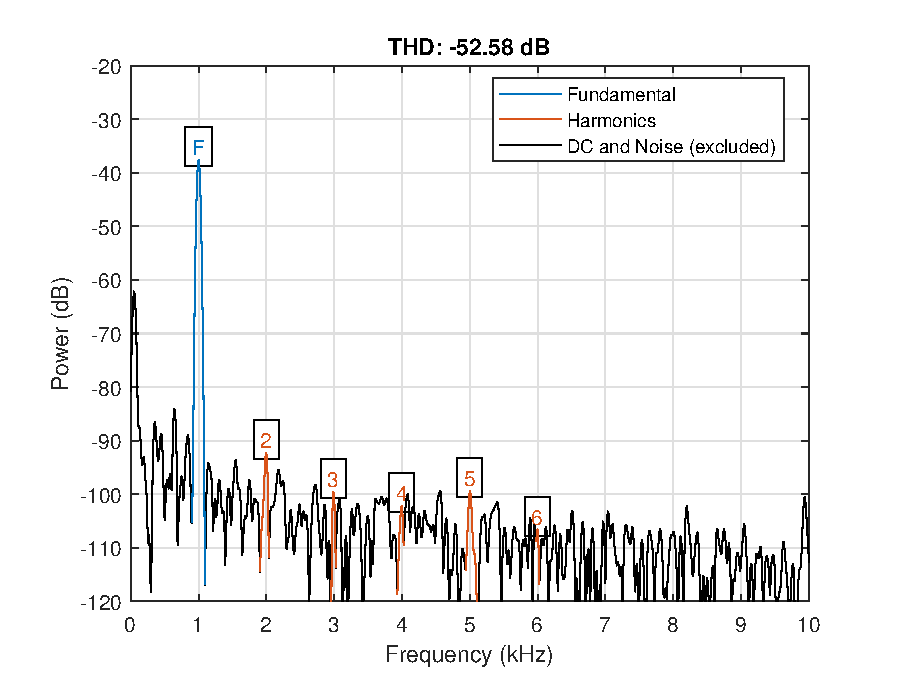
\includegraphics[scale=0.75]{./figs/dacTHDPlot.eps}        
    \caption{THD Plot of DAC}
    \label{fig:ti-thd}
\end{figure}

\begin{figure}[H]
    \centering
    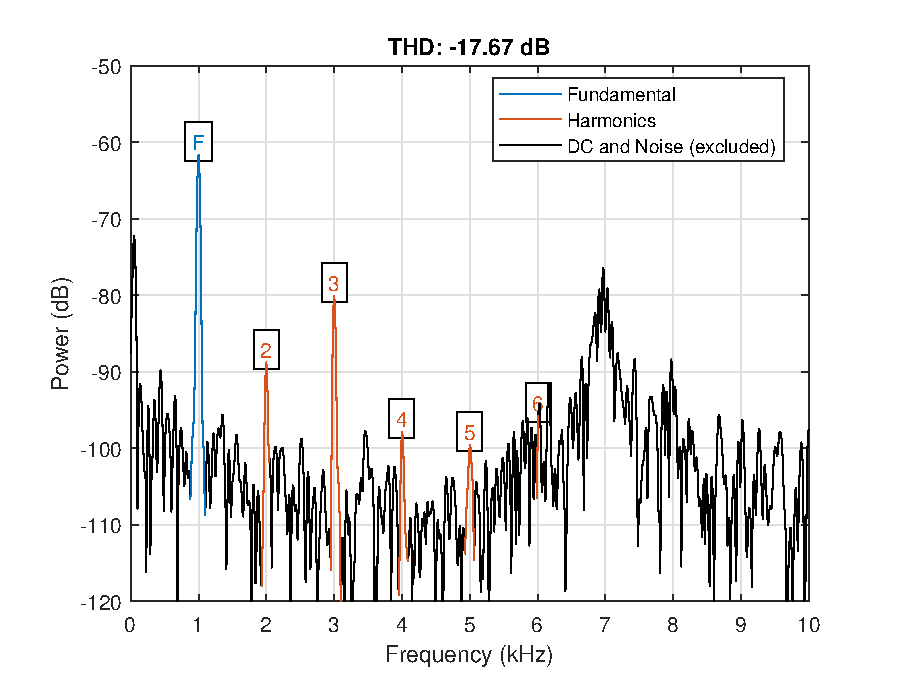
\includegraphics[scale=0.75]{./figs/maxiTHDPlot.eps}        
    \caption{THD Plot of Maxim}
    \label{fig:ti-thd}
\end{figure}

\begin{figure}[H]
    \centering
    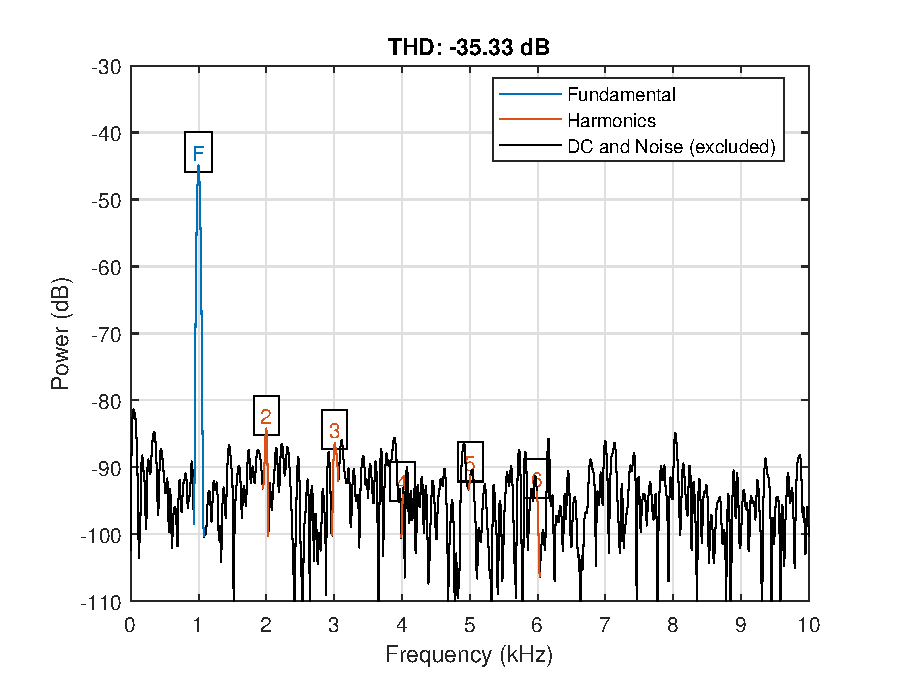
\includegraphics[scale=0.75]{./figs/tiTHDPlot.eps}        
    \caption{THD Plot of TI}
    \label{fig:ti-thd}
\end{figure}

\subsection{Discussion}

While the calculated values have a high variance from those observed in the datasheet, their results conform well to both the power analyser result measured from the DAC and the subjective experience of the listener. The single stage system shows extremely little harmonic response within the FFT as a result of the advanced digital signal processing elements it incorporates, which is reflected in the pure THD values. For greater confidence a dedicated signal analyser with class-d configurations would be required, however was not available within the scope of the project. 
\par 
At the project outset it was considered the single stage system may present too great a task to develop for without its associated evaluation module, however the use of the software packages provided by Texas Instruments greatly accelerated development. Future work would therefore move on with this system in favour of the dual stage, and could be improved by leveraging the configurable DSP within the chip to remove the strain of software filtering from the companion computer.

\end{document}